\section{Designing aSTEP-2020} \label{sc:tsinterface}
In section \ref{sc:astep2019}, we found that the UI, database, and server architecture are robust enough that they will need minimal or no redesigning. We also find the documentation format obscure, and in this section we propose a new format. Furthermore, we imagine that improvement could be made to the shared analytics platform.
\\\\
Our primary focus for \gls{astep}-2020 will, however, be to create an anomaly detection service for the data analytics platform.

\subsection{Documentation Service} \label{sc:docu_proposal}
We propose a new format for documentation through a new service. The format will consist of a Wiki-like service, incorporating the \gls{rfc}-list (with some changes to its purpose) as well as centralised documentation for all of \gls{astep}. Furthermore, we propose a change to the documentation shown directly in the interface.

\subsubsection{\gls{rfc}}
The \gls{rfc}-list will be moved to a Wiki-like service, and continue with some changes. Its focus will no longer be to provide documentation for the current implementation but instead will function as historical documentation of proposed changes to \gls{astep}, whether accepted or not. Each \gls{rfc} facilitates a timestamp for the proposal's creation, acceptance or rejection, and the last modification. Furthermore, each \gls{rfc} has a status (accepted/pending/rejected), and if rejected, the reasoning for rejection is described. The new \gls{rfc} list will help later semesters with decision making based on the history of proposals from the previous semesters.

\subsubsection{Shared Service/Guideline Documentation}
Documentation for shared services (such as the \gls{ui}, ServiceFetcher, etc.) will be moved to the Wiki-like service. This service should only contain documentation for current versions of implementation, and not serve as a historical reference.

\subsubsection{Service Documentation}
The new documentation format splits the service's documentation into "User Guide" and "Developer Documentation". The split in documentation will make it easier for an end-user to distinguish usage instructions as well as facilitate the extension of services by developers. The \gls{ui} will need to be changed slightly to facilitate this change. A Wiki page will contain developer documentation, and the individual services will display the Wiki page for the specific service.

\subsection{Shared Analytics Platform} \label{sc:sap}
Group SW606F20 proposes an addition to the \gls{ui} to facilitate inter-service communication better and shared analytics. This addition means that services must expose 2 additional \glspl{endpoint}, \textbf{/data}, \textbf{/combined}. \textbf{/data} must expose a service's output as raw data in JSON format. \textbf{/combined} will serve as a combination of \textbf{/render} and \textbf{/data}. Exposing a service's output, both as raw data and as a chart for rendering, will allow the \gls{ui} to use the output of one serving as the input to another. \textbf{/combined} will serve the purpose of both rendering the output of service, as well as using it as input to another. Figure \ref{fig:ui-addition} show a mock-up of the new interface.

\begin{figure}[htbp]
    \centering
    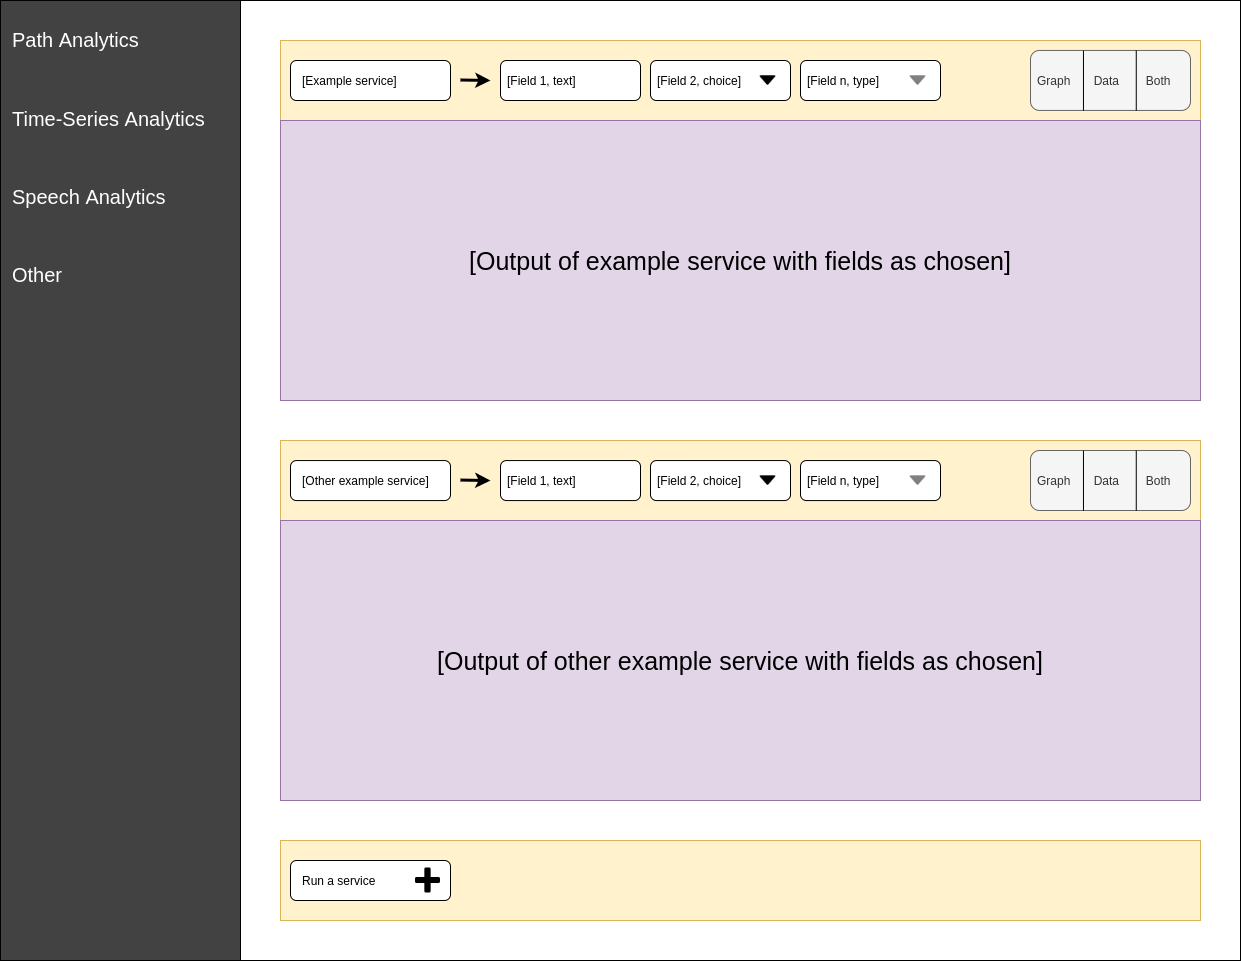
\includegraphics[width=0.8\textwidth]{Pictures/Sprint_1/single-interface.png}
    \caption{A mock-up of the addition to the \gls{astep} \gls{ui} made by group SW606F20.\cite{astep}}
    \label{fig:ui-addition}
\end{figure}

\subsection{Common Data Interface}
To further facilitate a shared analytics platform, group SW602F20 proposes a common data interface. This interface will allow the groups to work with the same data,  pass data from one service to another through the previously mentioned \gls{ui} addition. The data interface will allow the other groups to apply our anomaly detection solutions to their data before using it.
The time series subgroup decided a JSON-format would function as the data interface. Since the \gls{ui}, parses all data through JSON. Listing \ref{lst:common_interface} shows the interface.

\begin{listing}[htbp]
\begin{minted}[frame=single,
               framesep=3mm,
               linenos=true,
               xleftmargin=21pt,
               fontsize=\footnotesize,
               tabsize=4]{js}
{
  "dataSetName": "Name of dataset",
  "graphs": [
    {
      "label": "Name of graph",
      "data": [
        {
          "x": 2,
          "y": 35
        },
        {
          "x": 3,
          "y": 38
        }
      ]
    },
    {
      "label": "Name of graph",
      "data": [
        {
          "x": 5,
          "y": 33
        },
        {
          "x": 42,
          "y": 83
        },
        {
          "x": 56,
          "y": 153
        }
      ]
    }
  ]
}
\end{minted}
\caption{JSON for the common time series interface.} 
\label{lst:common_interface}
\end{listing}

The common data interface consists of several graphs, each with a label and some data points. Each data point must include an x-value and a y-value but may also include other data, such as a label for whether the point is an anomaly or not.